\chapter{Two Updates of YOLO-vf-seg}
\label{ch:methods}

The baseline defined in Section~\ref{sec:problem-gap} already proposes a mask and a center for each visible crate. This chapter adds the two computations that turn those proposals into a typed inventory. Section~\ref{sec:icph} derives the illumination-invariant chromatic prototype head. Section~\ref{sec:plc} derives perspective lattice completion. Each section states the quantity being computed, the reason a simpler quantity is the wrong one, the algorithm, the cost, and the way the module fails when its assumption fails. The numerical estimate is withheld until Chapter~\ref{ch:system}, where the observation model can be written next to the tables. A formula that appears in both places has the same meaning in both places.

\section{Illumination-invariant chromatic prototype head}
\label{sec:icph}

\subsection{Where the two modules sit on the forward pass}

Before either update is derived, the forward pass they attach to should be fixed in dimensions, so that ``a small head'' and ``a center'' are quantities rather than slogans. The pass described here is the YOLOv8-seg assembly with the vertical-feature gate of~\eqref{eq:vf}. It is the baseline. Nothing in this subsection is claimed as a contribution. The contributions begin at Section~\ref{sec:icph}.

An input frame is resized to the network's square working resolution, denoted $S\times S$ with three channels. The value of $S$ is a deployment choice, commonly $640$. The footprint calculation in Section~\ref{sec:footprint} shows that the lattice is not starved of pixels at the gate, so the reason to keep $S$ large is the lip between two stacked crates, not the metre-scale pitch. The backbone, a cross-stage convolutional network of the kind introduced for efficient gradient flow~\cite{wang2020cspnet} and used by the maintained YOLO implementations~\cite{jocher2023yolov8}, emits three maps whose strides are $8$, $16$, and $32$ pixels. On a $640$ input those maps are $80\times 80$, $40\times 40$, and $20\times 20$. The neck builds the feature pyramid~\cite{lin2017fpn} and, on each of the three maps, applies the vertical gate
\begin{equation}
a = \sigma\!\left( g(\operatorname{GAP}_{w}(U)) \right),
\qquad
\tilde U_{c,i,j} = a_{c,i}\, U_{c,i,j}.
\label{eq:vf-again}
\end{equation}
The pooled column $\operatorname{GAP}_{w}(U)$ has shape $C\times H\times 1$. A convolution of kernel $1\times 3$ along $H$ mixes each row with the lip above it and the lip below it, which is the only place in the baseline where the stack's periodicity is written down as an architectural bias. The sigmoid keeps the gate in $(0,1)$ so that a row can be suppressed and cannot be amplified without bound. A row that contains a horizontal lip receives a larger $a$ if $g$ learns to respond to the vertical gradient of the pooled column. A row that contains only the flat plastic of a crate face receives a smaller $a$. The gate does not know the pitch in metres. It knows only that the informative variation, on this camera, runs down the image.

The detection head is decoupled. At each spatial site and at each stride it predicts an objectness, a class distribution over whatever classes the segmenter was trained to emit, and a box. For the brewery the segmenter's class may be the single class ``crate.'' Color is not this distribution. Color is ICPH, precisely so that a change of lamp does not have to be solved by the same softmax that decides whether a site is a crate. The box is parameterized as an offset from the site center plus a width and a height, the anchor-free form used since YOLOX~\cite{ge2021yolox}. Non-maximum suppression then keeps one box when two sites describe the same crate. The surviving box is the window inside which the mask is cropped, and its center is the fallback center if the mask is empty. The mask head, in parallel, predicts $K_{p}=32$ prototype masks at stride $4$, so on a $640$ input the prototypes are $160\times 160$, and one coefficient vector $c\in\mathbb{R}^{32}$ per detection. The mask is~\eqref{eq:yolact}, cropped to the box and thresholded at one half. The center passed to PLC is the first moment of the thresholded mask,
\begin{equation}
\bar u = \frac{\sum_{x\in M} u(x)}{\lvert M\rvert},
\qquad
\bar v = \frac{\sum_{x\in M} v(x)}{\lvert M\rvert},
\label{eq:moment}
\end{equation}
then mapped by $H$. Using the moment rather than the box center lets a crate that is half in shadow pull its reported center toward the visible plastic, which is usually toward the interior of the stack rather than toward the aisle. That pull is helpful when the shadow is on the outside of the face and harmful when the shadow is the seam, because the moment then slides toward the neighbor. The $3.5\,\mathrm{cm}$ noise in the counting model is a stand-in for both effects. It is not a measurement of~\eqref{eq:moment} on real masks.

ICPH reads $M$ and, in the full specification, the mask-pooled vector~\eqref{eq:pool} from the finest neck map. It does not read the prototype coefficients. Those coefficients are a spatial code, shared in meaning with YOLACT's prototypes~\cite{bolya2019yolact}, and they are not a color. Reusing $c$ as a color feature would entangle the seam with the lamp. The head's output is a class and a margin, attached to the same index as the center, so that cell $(r,c)$ and class $\hat k$ refer to one detection until the gap rule invents a cell that has no detection. Invented cells are the only ones that inherit a class, by the neighbor rule in~\eqref{eq:per-color}.

\begin{figure}[t]
\centering
\begin{tikzpicture}[
  font=\footnotesize,
  box/.style={draw, rounded corners=1.5pt, align=center, inner sep=3pt, minimum height=8mm, minimum width=18mm},
  arr/.style={-{Stealth}, semithick}
]
  \node[box, fill=black!6] (in) {Image\\$S\times S\times 3$};
  \node[box, fill=black!6, right=4mm of in] (bb) {Backbone\\strides 8, 16, 32};
  \node[box, fill=blue!10, right=4mm of bb] (vf) {Vertical gate\\on each level};
  \node[box, fill=black!6, right=4mm of vf] (det) {Decoupled\\boxes};
  \node[box, fill=black!6, below=7mm of det] (msk) {32 prototypes\\and coefficients};
  \node[box, fill=orange!15, below=7mm of vf] (icph) {ICPH\\class, margin};
  \node[box, fill=green!12, below=7mm of bb] (plc) {PLC\\cells $\times$ depth};
  \draw[arr] (in) -- (bb);
  \draw[arr] (bb) -- (vf);
  \draw[arr] (vf) -- (det);
  \draw[arr] (det) -- (msk);
  \draw[arr] (msk) -- (icph);
  \draw[arr] (msk.west) -- ++(-2mm,0) |- (plc.east);
  \node[align=center, font=\scriptsize] at ($(msk.west)+(-1.15,-0.55)$) {centers};
  \node[align=center, font=\scriptsize] at ($(msk.south)+(0,-0.45)$) {pixels in $M$};
\end{tikzpicture}
\caption{Forward pass of the updated model. The backbone and the vertical gate are the baseline YOLO-vf-seg. The prototype assembly produces the mask. ICPH and PLC both read that mask and do not read each other. Depth enters PLC from outside the figure.}
\label{fig:forward}
\end{figure}

The cost of being this explicit is that several widely discussed alternatives are now visibly in the wrong place. A second class head on the detection branch would name the color from the box features, including background inside the box, and would be trained by the same assignment that trains objectness. ICPH is downstream of the mask so that the pixels are the crate. A density head on the pyramid would estimate a visible count and would never see $\hat d$. PLC is downstream of the centers so that the pitch can be applied in metres. A global constancy preprocessing in front of the backbone would rescale the whole frame before the gate saw it, and \Cref{prop:uniform} says a per-face rescaling is already destructive if it is used as the classifier. No constancy step sits in front of the backbone. The camera gain is locked, and the only place an illuminant is estimated is inside $M$, as one block of $\mathbf{f}$.

The numbers that a deployer tunes, and that this thesis does not claim to have tuned on images, are $S$, the non-maximum-suppression overlap, the mask threshold of one half, and $K_{p}$. Moving $K_{p}$ from $32$ to $16$ halves the prototype tensor and, on COCO-like masks, usually costs a small amount of boundary detail~\cite{bolya2019yolact,zhao2023fastsam}. On a crate face the boundary that matters is one horizontal lip. Whether $16$ prototypes can express that lip is a question for a labeled gate, not for the Monte Carlo model, which never renders a lip. The model begins at the center. The architecture above is what has to produce a center that \Cref{prop:snap} can trust.


\subsection{The decision the head is asked to make}
\label{sec:icph-decision}

Let $M\subset\Omega$ be the set of pixels that the segmenter has marked as one crate, and let $\mathbf{I}(x)$ be the observed color at those pixels. ICPH returns a class $\hat{k}\in\mathcal{K}$ with $\lvert\mathcal{K}\rvert=6$, the six body colors of \Cref{ass:color}. It does not return a corrected image, and it does not return an illuminant for the whole frame. The inventory needs a name per mask. Anything else the head computes is an intermediate that exists to make that name stable.

The head is attached where the mask already exists, for a reason that is easy to understate. A color decision taken on a box, rather than on a mask, mixes the crate with the background that the box contains: the gap between slats, a piece of the crate behind, the forks at the bottom row. A color decision taken on the whole frame mixes every crate on the pallet. The mask is the smallest region for which \Cref{ass:color} is even approximately true. ICPH therefore refuses to run on a detection that has no mask. If the segmenter emits only a box, the system falls back to the raw prototype match described below and marks the type as low confidence. That fallback is a degradation, not the design.

\begin{figure}[t]
\centering
\begin{tikzpicture}[
  font=\small,
  box/.style={draw, rounded corners=2pt, align=center, inner sep=4pt, minimum height=7.5mm, fill=orange!10},
  arr/.style={-{Stealth}, thick}
]
  \node[box] (mask) {Mask $M$\\and pixels $\mathbf{I}(M)$};
  \node[box, right=7mm of mask] (mink) {Minkowski\\norm, order $p{=}6$};
  \node[box, right=7mm of mink] (feat) {Feature $\mathbf{f}\in\mathbb{R}^{8}$\\$\chi$, $o$, $\eta$};
  \node[box, fill=blue!8, below=8mm of feat] (std) {Standardize\\with training $\mu,\sigma$};
  \node[box, fill=blue!8, left=7mm of std] (lin) {Linear scores\\$W\tilde{\mathbf{f}}+b$};
  \node[box, fill=green!12, left=7mm of lin] (cls) {Class $\hat{k}$\\and margin};
  \draw[arr] (mask) -- (mink);
  \draw[arr] (mink) -- (feat);
  \draw[arr] (feat) -- (std);
  \draw[arr] (std) -- (lin);
  \draw[arr] (lin) -- (cls);
  \node[box, fill=black!5, below=7mm of mask] (pool) {Optional neck vector\\mask-pooled, 256-d};
  \node[box, fill=black!5, below=7mm of lin] (proj) {Projection to 32-d\\residual path};
  \draw[arr] (pool) -- (proj);
  \draw[arr] (proj) -- (lin);
\end{tikzpicture}
\caption{ICPH on one mask. The upper path is the chromatic feature that the estimate in Chapter~\ref{ch:system} actually trains. The lower path is the mask-pooled neck vector specified for the full segmenter. The linear layer is the prototype score. Both paths are cheap relative to the backbone.}
\label{fig:icph-block}
\end{figure}

\subsection{A per-mask illuminant that must not be trusted alone}
\label{sec:icph-illum}

Inside $M$ the diagonal model~\eqref{eq:diagonal} still applies, with one extra scalar. Shading and exposure multiply every channel by a positive $s(x)$, so
\begin{equation}
\mathbf{I}(x) = s(x)\, \mathbf{L} \odot \mathbf{R},
\qquad x\in M,
\label{eq:shaded}
\end{equation}
where the reflectance $\mathbf{R}$ has been pulled out of the pixel index because \Cref{ass:color} says the body is one color. Logos and drainage slots violate that pull-out on a small set of pixels. The head does not try to segment the logo. It relies on the Minkowski norm with $p>1$ to reduce the influence of the darkest slots, and on the training contamination described in Section~\ref{sec:icph-train} to see a strip of the neighboring crate.

The shades-of-gray estimate on the mask is~\eqref{eq:minkowski} with $\Omega=M$ and $p=6$:
\begin{equation}
\hat{\ell}_c
= \left(
\frac{1}{\lvert M\rvert}
\sum_{x\in M} \lvert I_c(x)\rvert^{6}
\right)^{1/6},
\qquad
\hat{\ell}_c \ge \varepsilon,
\label{eq:sog-mask}
\end{equation}
with $\varepsilon=10^{-6}$ only to avoid a division by zero on a degenerate mask. The corrected pixels are $\mathbf{I}'(x)=\mathbf{I}(x)\oslash\hat{\ell}$.

\begin{proposition}[A uniform face has no illuminant residual]
\label{prop:uniform}
Suppose $s(x)=s$ is constant on $M$ and $\mathbf{I}(x)=s\,\mathbf{L}\odot\mathbf{R}$ for every $x\in M$. Then $\hat{\ell}$ is parallel to $\mathbf{L}\odot\mathbf{R}$, the corrected color $\mathbf{I}'$ is constant across channels up to the common scale, and the chromaticity of $\mathbf{I}'$ is $(1/3,1/3,1/3)$ whenever no channel of $\mathbf{L}\odot\mathbf{R}$ is zero.
\end{proposition}

\begin{proof}
Under the hypothesis every pixel is the same vector $\mathbf{v}=s\,\mathbf{L}\odot\mathbf{R}$. The Minkowski norm of a constant set is the absolute value of that constant, so $\hat{\ell}=\lvert\mathbf{v}\rvert$ element-wise. Division by $\hat{\ell}$ yields a vector of ones on every channel that was nonzero. Its chromaticity, the normalization by the sum of channels, is the neutral point.
\end{proof}

\Cref{prop:uniform} is the reason ICPH does not classify $\mathbf{I}'$. On a clean crate face the classical correction succeeds at removing the illuminant and, in the same division, succeeds at removing the reflectance. Gray-world ($p=1$) and shades-of-gray ($p=6$) fail in the same direction. The failure is slightly worse for larger $p$ only because a larger $p$ concentrates on the brightest pixels, which on a uniform face are the same color as the mean. The estimate in Chapter~\ref{ch:system} is where this proposition becomes a table: both classical corrections fall to roughly one fifth accuracy, which is little above the one-in-six rate of a guess among six colors, as soon as the face is close to uniform.

The proposition also says where a residual can come from. If $s(x)$ varies, if a fraction of $M$ belongs to a neighbor, or if a logo has a different reflectance, then $\hat{\ell}$ is no longer parallel to a single $\mathbf{L}\odot\mathbf{R}$ and $\mathbf{I}'$ is no longer neutral. Those violations are exactly the nuisances of the passage. They are weak signals. A method that needs them in order to retain any color at all is a method that has thrown away $\mathbf{R}$. ICPH therefore keeps three views of the same pixels at once: the corrected chromaticity, which is informative when the mask is contaminated; the opponent coordinates of that chromaticity, which align with the amber--yellow and red--green confusions; and the chromaticity of $\hat{\ell}$ itself, which still carries $\mathbf{L}\odot\mathbf{R}$ and is the term the classical correction divides out.

\subsection{The eight-dimensional feature}
\label{sec:icph-feature}

Let $\bar{\mathbf{I}}'$ be the mean of the corrected pixels on $M$. Chromaticity drops the intensity:
\begin{equation}
\chi
= \frac{\bar{\mathbf{I}}'}{\mathbf{1}^{\top}\bar{\mathbf{I}}'+\varepsilon}
\in\mathbb{R}^{3}.
\label{eq:chroma}
\end{equation}
The opponent pair used here is the simplest linear map that separates red from green and that pair from blue,
\begin{equation}
o_{1}=\chi_{r}-\chi_{g},
\qquad
o_{2}=\tfrac{1}{2}(\chi_{r}+\chi_{g})-\chi_{b}.
\label{eq:opponent}
\end{equation}
The illuminant feature is the chromaticity of the Minkowski estimate, not its magnitude. Magnitude is brightness, and brightness is the fork shadow:
\begin{equation}
\eta
= \frac{\hat{\ell}}{\mathbf{1}^{\top}\hat{\ell}+\varepsilon}
\in\mathbb{R}^{3}.
\label{eq:eta}
\end{equation}
The head concatenates them,
\begin{equation}
\mathbf{f}
= \begin{bmatrix} \chi \\ o \\ \eta \end{bmatrix}
\in\mathbb{R}^{8}.
\label{eq:feature}
\end{equation}
\Cref{alg:feature} is the same construction in the order the implementation uses.

\begin{algorithm}[t]
\caption{Chromatic feature of one mask}
\label{alg:feature}
\begin{algorithmic}[1]
\Require pixels $\{\mathbf{I}(x):x\in M\}$, order $p=6$, floor $\varepsilon=10^{-6}$
\State $\hat{\ell}_c \gets \big(\lvert M\rvert^{-1}\sum_{x\in M}\lvert I_c(x)\rvert^{p}\big)^{1/p}$ for each channel $c$
\State $\hat{\ell} \gets \max(\hat{\ell},\varepsilon)$
\State $\mathbf{I}'(x) \gets \mathbf{I}(x)\oslash\hat{\ell}$
\State $\chi \gets \operatorname{mean}(\mathbf{I}') / (\mathbf{1}^{\top}\operatorname{mean}(\mathbf{I}')+\varepsilon)$
\State $o \gets (\chi_r-\chi_g,\ \tfrac{1}{2}(\chi_r+\chi_g)-\chi_b)$
\State $\eta \gets \hat{\ell}/(\mathbf{1}^{\top}\hat{\ell}+\varepsilon)$
\State \Return $\mathbf{f}\gets[\chi;\,o;\,\eta]$
\end{algorithmic}
\end{algorithm}

Two normalizations are doing different jobs and should not be collapsed. Division by $\hat{\ell}$ inside $\mathbf{I}'$ is a color-constancy step, and \Cref{prop:uniform} says it is destructive when it is used alone. Division by the channel sum inside $\chi$ and $\eta$ removes intensity after that step. The opponent map is not a normalization. It is a choice of axes. Amber and yellow differ mostly along a red--green direction that has been rotated slightly toward yellow; $o_1$ is a coarse version of that axis, not a perceptual uniform space. A more careful uniform color space would be justified if the prototypes were close. They are not close in the nominal palette. They become close only after a strong illuminant has moved the observations, which is the regime the linear classifier is trained for.

The nominal reflectances used to build the palette, written as linear RGB triples, are
\begin{equation}
\begin{aligned}
\mathbf{R}_{\text{amber}}&=(0.72,0.45,0.12),&
\mathbf{R}_{\text{green}}&=(0.15,0.55,0.22),&
\mathbf{R}_{\text{red}}&=(0.70,0.12,0.12),\\
\mathbf{R}_{\text{blue}}&=(0.12,0.25,0.62),&
\mathbf{R}_{\text{yellow}}&=(0.85,0.75,0.15),&
\mathbf{R}_{\text{white}}&=(0.82,0.82,0.80).
\end{aligned}
\label{eq:prototypes}
\end{equation}
These are design values, chosen to be separable in chromaticity and to resemble the families of returnable crates, not spectrophotometric measurements of a named manufacturer. Their chromaticities already predict the confusions. Amber and yellow both have a small blue coordinate and a large red coordinate. White is near $(1/3,1/3,1/3)$. Red and blue are far from everyone. The estimate later shows that pattern in the harsh-illuminant confusion matrix rather than as a surprise.

\begin{figure}[t]
\centering
\begin{tikzpicture}
\begin{axis}[
  width=0.78\textwidth,
  height=7.2cm,
  xlabel={$\chi_r$},
  ylabel={$\chi_g$},
  xmin=0, xmax=0.9,
  ymin=0, ymax=0.75,
  legend pos=north east,
  tick label style={font=\small},
  label style={font=\small},
  legend style={font=\small}
]
\addplot[only marks, mark=*, mark size=2.5pt] coordinates {
  (0.558,0.349)
  (0.163,0.598)
  (0.745,0.128)
  (0.121,0.253)
  (0.486,0.429)
  (0.336,0.336)
};
\node[font=\small, anchor=west] at (axis cs:0.558,0.349) {amber};
\node[font=\small, anchor=north west] at (axis cs:0.17,0.59) {green};
\node[font=\small, anchor=west] at (axis cs:0.745,0.128) {red};
\node[font=\small, anchor=west] at (axis cs:0.121,0.253) {blue};
\node[font=\small, anchor=south west] at (axis cs:0.486,0.429) {yellow};
\node[font=\small, anchor=east] at (axis cs:0.336,0.336) {white};
\end{axis}
\end{tikzpicture}
\caption{Chromaticity of the six design prototypes~\eqref{eq:prototypes}, plotted in the $(\chi_r,\chi_g)$ plane. Blue is omitted from the third coordinate and is small for amber and yellow, which is why those two classes approach each other when the illuminant estimate is noisy. White sits near the neutral point.}
\label{fig:chroma-plane}
\end{figure}

\subsection{Scores against prototypes}
\label{sec:icph-score}

A training set of features is standardized with the coordinate-wise mean $\mu\in\mathbb{R}^{8}$ and standard deviation $\sigma\in\mathbb{R}^{8}$ of that set,
\begin{equation}
\tilde{\mathbf{f}} = (\mathbf{f}-\mu)\oslash\sigma.
\label{eq:standardize}
\end{equation}
The score of class $k$ is linear,
\begin{equation}
z_k = W_{k,:}\,\tilde{\mathbf{f}} + b_k,
\qquad
W\in\mathbb{R}^{6\times 8}.
\label{eq:linear}
\end{equation}
The predicted class and the margin are
\begin{equation}
\hat{k}=\argmax_k z_k,
\qquad
\gamma = z_{\hat{k}} - \max_{k\neq\hat{k}} z_k.
\label{eq:margin}
\end{equation}
The margin is part of the product, not a training detail. A passage that contains one low-margin crate should be flagged for the operator even when the lattice is confident, because a swap of amber and yellow does not change the geometry that PLC checks. The system rule is given in Section~\ref{sec:sys-output}. The head itself only computes $\gamma$.

The training loss on a labeled feature is the cross-entropy of the softmax, plus an $\ell_2$ penalty on $W$,
\begin{equation}
\mathcal{L}
= -\log \softmax(z)_{y}
+ \frac{\lambda}{2}\lVert W\rVert_{F}^{2},
\label{eq:loss}
\end{equation}
with $\lambda=10^{-3}$ in the estimate. There is no penalty on $b$. The softmax is the usual one,
\begin{equation}
\softmax(z)_k
= \frac{\exp(z_k)}{\sum_{j\in\mathcal{K}}\exp(z_j)}.
\label{eq:softmax}
\end{equation}
This is a linear classifier on a hand-built feature. It is not a second detection network. The justification for stopping at a linear map is the dimension: eight coordinates, six classes, and a feature that was constructed so that the classes are roughly linear in it. If a field trial shows a curved boundary between amber and yellow, the replacement is a small multilayer perceptron on the same $\mathbf{f}$. The interface, the mask in and the class out, does not change.

The raw-RGB baseline that the estimate compares against ignores illumination. It takes the mean pixel $\bar{\mathbf{I}}$ on the mask, normalizes it to unit length, and chooses the prototype of nearest cosine,
\begin{equation}
\hat{k}_{\text{raw}}
= \argmax_{k\in\mathcal{K}}
\frac{\mathbf{R}_{k}^{\top}\bar{\mathbf{I}}}{\lVert\mathbf{R}_{k}\rVert\,\lVert\bar{\mathbf{I}}\rVert}.
\label{eq:raw}
\end{equation}
The gray-world and shades-of-gray baselines correct the pixels first, with $p=1$ and $p=6$, and then apply the same nearest-prototype rule to the corrected mean. Under \Cref{prop:uniform} those two baselines are predicted to collapse. The raw rule is predicted to be strong when $\mathbf{L}$ is near the white point and to decay as the random gain in the observation model grows. ICPH is predicted to decay more slowly, because $\eta$ still carries the direction of $\mathbf{L}\odot\mathbf{R}$ and the classifier can learn to read it. Chapter~\ref{ch:system} is where those predictions are checked. They are predictions about a model, and they are stated here so that the table cannot be mistaken for an exploration that found a pattern after the fact.

\subsection{The neck path that the full segmenter adds}
\label{sec:icph-neck}

The chromatic feature does not see the logo as a spatial pattern, and it does not see the difference between a crate face and a printed label of the same average color. The full head specified for YOLO-vf-seg therefore adds the mask-pooled neck vector. Let $U$ be the finest neck map that still has a channel count of $256$, and let $\Pi(M)$ be the set of spatial indices of $U$ that fall inside $M$. Mask pooling is
\begin{equation}
\mathbf{u}
= \frac{1}{\lvert\Pi(M)\rvert}
\sum_{q\in\Pi(M)} U_{q}
\in\mathbb{R}^{256}.
\label{eq:pool}
\end{equation}
A pointwise projection $P_{32}\in\mathbb{R}^{32\times 256}$ and a bias produce a 32-dimensional embedding. In parallel, a small perceptron maps the three raw channel means of the mask through a hidden width of 32 and out to the six classes, and that path is added to the linear scores of~\eqref{eq:linear}. The parameter count of this specification is
\begin{equation}
\begin{aligned}
N_{\text{proj}} &= 256\cdot 32 + 32,\\
N_{\text{mlp}} &= 3\cdot 32 + 32\cdot 32 + 32 + 32\cdot 6,\\
N_{\text{proto}} &= 32\cdot 6,\\
N_{\text{ICPH}} &= N_{\text{proj}}+N_{\text{mlp}}+N_{\text{proto}} = 9760,
\end{aligned}
\label{eq:params}
\end{equation}
where the prototype term counts a $32\times 6$ cosine table and the MLP term counts the illuminant residual path used in the cost model. Relative to a YOLOv8m-seg reference of $27.3\times 10^{6}$ parameters, the fraction is $3.6\times 10^{-4}$. The FLOPs of the head are one pooled vector per detection. They do not change the leading term of the segmenter, which for that reference model is on the order of $10^{2}$ GFLOPs. The estimate records the fraction and does not claim a new timing measurement on a device.

The split between what is trained in the estimate and what is specified for the system is deliberate. The Monte Carlo instrument trains~\eqref{eq:linear} on~\eqref{eq:feature}. It does not train a YOLO backbone, because no labeled passage images are part of this thesis. The neck path is specified so that a later training run on real frames has a place to put appearance that is not a global color, and so that the parameter budget is fixed before that run. Reporting the chromatic-path accuracy as if it were the full neck-path accuracy would be a misstatement. Chapter~\ref{ch:system} repeats the distinction next to the table.

\subsection{How the training distribution is built}
\label{sec:icph-train}

Each training face is drawn as follows. A class $k$ is uniform on the six prototypes. An illuminant gain is drawn as a log-normal vector,
\begin{equation}
\mathbf{g} = \exp(\boldsymbol{\xi}),
\qquad
\xi_c \sim \mathcal{N}(0,s^{2}),
\qquad
\mathbf{g}\gets \mathbf{g}/\operatorname{mean}(\mathbf{g}),
\label{eq:gain}
\end{equation}
with severity $s$ uniform between $0.05$ and $0.55$ during training. The normalization by the mean removes a pure exposure change, which shading already models, and keeps the draw on the illuminant direction. A shadow scalar $\rho$ is uniform on $[0.40,1]$, and a smooth shade multiplies the rows of the patch by a line from $0.72$ to $1.18$. With probability $0.25$ the first $18$ percent of the rows are replaced by a different prototype under the same $\mathbf{g}$ and $\rho$, which is the neighboring-crate strip. Pixel noise of standard deviation $0.012$ is added and negative values are clipped. The feature~\eqref{eq:feature} is computed on that patch, and the label is $k$.

Six thousand patches and five hundred full-batch gradient steps with step size $0.35$ are the training schedule of the estimate. The step size is large because the features are standardized and the model is linear; it is not a step size that would be copied onto a YOLO backbone. The $\ell_2$ penalty is applied to $W$ on every step. Nothing in this schedule is claimed to be optimal. It is fixed, it is seeded, and the test patches are drawn after training from the same generative steps at fixed severities that training never isolated.

The strip of a neighbor is the important augmentation. Without it the classifier can ignore $\chi$ and read the class from $\eta$ alone, because on a pure face $\eta$ is the chromaticity of $\mathbf{L}\odot\mathbf{R}$. With the strip, $\eta$ is pulled toward the neighbor and $\chi$ carries the disagreement between the two reflectances. That disagreement is what a real mask boundary looks like. Training without the strip would overstate accuracy on clean faces and understate the amber--yellow collision when the boundary is wrong.

\subsection{Calibration of the margin}
\label{sec:icph-margin}

The margin $\gamma$ in~\eqref{eq:margin} is not a probability. Softmax outputs of a linear model trained under a single generative severity are not calibrated to a different severity, and a warehouse shift is exactly a change of severity. The system therefore treats $\gamma$ as a rank, not as a chance. The operating rule, justified by the harsh-severity confusion in Chapter~\ref{ch:system}, is:

\begin{itemize}
\item if $\gamma$ is among the lowest tenth of margins seen on a calibration shift, the type is marked uncertain;
\item uncertain types are excluded from the automatic per-color tally and listed for the operator;
\item the total count from PLC is still reported, because geometry does not depend on $\gamma$.
\end{itemize}

A calibration shift is a few dozen pallets of known color at the start of a week, not a gray card. This is the one place the design asks a person to confirm a label. It is also the place where amber and yellow will concentrate if the lamps in that building are worse than the harsh setting of the estimate. The rule is a consequence of \Cref{prop:uniform} being only approximately false: when the residual that ICPH reads becomes small, the honest output is an abstention, not a forced name.

\subsection{Cost, interfaces, and the failures that remain}
\label{sec:icph-cost}

The runtime interface is a mask and a patch of pixels in, and a class plus a margin out. The training interface is a set of patches drawn as in Section~\ref{sec:icph-train}, or, when real images exist, the same feature computed on masks whose color a person has confirmed. The head does not modify the mask and does not modify the lattice. Those two statements are what keep the estimate separable. A color error cannot create a cell, and a gap-fill cannot change a prototype.

The failures that the derivation predicts, and that the estimate should be checked against, are the following.

\begin{enumerate}
\item At very small severity the raw cosine~\eqref{eq:raw} can beat ICPH, because the correction inside $\chi$ removes a reflectance signal that the raw matcher was using lawfully. A crossover at low severity is not a defect of the table. It is \Cref{prop:uniform} in mild form.
\item Amber and yellow remain the nearest pair. No linear feature built from a three-channel mean separates them once the gain noise exceeds their chromatic distance. More pixels do not help if the pixels are the same color. A logo-aware neck path might help. The chromatic path alone will not finish the job.
\item White is near neutral. Any error in $\hat{\ell}$ moves $\eta$ toward a chromatic class, and white is then confused with several classes rather than with one neighbor. The confusion matrix should show a white row that is spread out, not a white row that is swapped with a single partner.
\item A mask that contains more of the neighbor than of the crate will be classified as the neighbor. ICPH does not repair a bad mask. The segmenter remains responsible for $M$.
\end{enumerate}

These four points are the contract between this section and the color table. A result that contradicted them would mean the observation model and the head were not implementing the same mathematics. A result that matches them is evidence about the model, which is all a Monte Carlo estimate can be.

\subsection{Worked feature on two prototypes}
\label{sec:icph-worked}

The algebra is easier to see on a single pixel with no shade and no strip. Take a unit-mean illuminant $\mathbf{L}=(1.20,0.90,0.90)$ and the amber prototype. The observed color is
\begin{equation}
\mathbf{I}
= (1.20\cdot 0.72,\ 0.90\cdot 0.45,\ 0.90\cdot 0.12)
= (0.864,\ 0.405,\ 0.108).
\label{eq:worked-i}
\end{equation}
The Minkowski norm of a single pixel is the pixel, so $\hat{\ell}=\mathbf{I}$ and the corrected color is $(1,1,1)$. Chromaticity $\chi$ is neutral and both opponent coordinates are zero. The illuminant feature $\eta$ is the chromaticity of $\mathbf{I}$ itself,
\begin{equation}
\eta
= \frac{(0.864,0.405,0.108)}{1.377}
= (0.628,\ 0.294,\ 0.078).
\label{eq:worked-eta}
\end{equation}
The raw matcher sees $\mathbf{I}$, which is exactly $\mathbf{L}\odot\mathbf{R}_{\text{amber}}$, and still matches amber if no other prototype is closer after the gain. The classical corrected matcher sees white. ICPH sees a neutral $\chi$ and an $\eta$ that still points at amber under this lamp. That is the entire content of the head on a clean face: do not divide the reflectance away and then hope the classifier reconstructs it.

Now replace the blue channel's observation by a contamination, $\mathbf{I}=(0.864,0.405,0.250)$, as if a small amount of a brighter neighbor had entered the mean. Then $\hat{\ell}$ changes, $\chi$ leaves the neutral point, and $o_{2}$ becomes negative because the blue coordinate of $\chi$ rises. The linear layer has a coordinate, $o_2$, on which that contamination is visible. Whether the layer uses it is what the gradient steps decide. The hand calculation only shows that the coordinate exists, which \Cref{prop:uniform} says it does not exist on a pure face.

\subsection{What each block of the feature is worth}
\label{sec:icph-ablation}

\Cref{prop:uniform} says that $\chi$ and $o$ go to zero on a pure face, and that $\eta$ keeps $\mathbf{L}\odot\mathbf{R}$. The linear layer might still use the small residuals that shading and the neighbor strip leave in $\chi$. Whether it does is an empirical question about this feature, and it can be asked inside the same generator without a new theory. A second run, restarted from the same seed and the same schedule of six thousand patches and five hundred steps, trains six classifiers. Each classifier sees a subset of the eight coordinates. The subsets are the three chromaticity coordinates, the two opponent coordinates, the three illuminant coordinates, chromaticity with opponent, chromaticity with illuminant, and the full vector. Accuracy is measured at severities $0.05$, $0.30$, and $0.60$ on $2500$ fresh patches each. This run is not the run behind \Cref{tab:color}. Restarting the seed consumes the random stream in a different order, so the full-feature column here is a replicate, not a transcription.

\begin{table}[t]
\centering
\caption{Top-1 accuracy of linear heads trained on subsets of $\mathbf{f}$. The full row is a replicate of the ICPH feature, not the main table. Chance is $1/6\approx 0.167$.}
\label{tab:ablation}
\small
\begin{tabular}{@{}lccc@{}}
\toprule
Coordinates & $s=0.05$ & $s=0.30$ & $s=0.60$ \\
\midrule
Chromaticity $\chi$ only & $0.542$ & $0.534$ & $0.486$ \\
Opponent $o$ only & $0.538$ & $0.529$ & $0.480$ \\
Illuminant $\eta$ only & $0.864$ & $0.705$ & $0.504$ \\
$\chi$ and $o$ & $0.550$ & $0.532$ & $0.494$ \\
$\chi$ and $\eta$ & $0.976$ & $0.824$ & $0.592$ \\
Full $\mathbf{f}$ & $0.974$ & $0.827$ & $0.596$ \\
\bottomrule
\end{tabular}
\end{table}

\Cref{tab:ablation} is the practical form of the proposition. Chromaticity alone, the quantity a corrected matcher would trust, sits near $0.54$ at a mild lamp and falls toward $0.49$ at a harsh one. It is well above chance, because the shade ramp and the neighbor strip keep $\chi$ from being exactly neutral, and it is far below the raw matcher, which at low severity still sees $\mathbf{R}$ directly. Opponent coordinates alone do no better. They are a rotation of $\chi$, and a rotation cannot recover a signal the correction destroyed. Adding opponent to chromaticity moves the mild-lamp accuracy from $0.542$ to $0.550$. The opponent block is not where the accuracy lives.

The illuminant block alone is a different estimator. At $s=0.05$ it reaches $0.864$. On a nearly pure face $\eta$ is the chromaticity of $\mathbf{L}\odot\mathbf{R}$, and when $\mathbf{L}$ is near white that chromaticity is nearly the chromaticity of $\mathbf{R}$. At $s=0.60$ the same block falls to $0.504$, close to chromaticity-only. A strong gain rotates $\mathbf{L}\odot\mathbf{R}$ off the prototype, and $\eta$ rotates with it. The illuminant feature is a good feature exactly while the lamp is the nuisance the raw matcher can also tolerate, and it ceases to be sufficient at the severity ICPH was introduced to handle.

The combination of $\chi$ and $\eta$ is the head. At $s=0.05$ it reaches $0.976$, at $s=0.30$ it reaches $0.824$, and at $s=0.60$ it reaches $0.592$. The full eight-dimensional vector changes those three numbers to $0.974$, $0.827$, and $0.596$. Opponent coordinates are worth a few thousandths at the harsh end and a slight loss at the mild end, which is what an almost-redundant linear feature does under an $\ell_2$ penalty. They are kept in the specified head because they cost two coordinates and because the amber--yellow axis is an opponent axis. They are not kept because the ablation shows a large effect. A deployment that needs to shrink the feature can drop $o$ and expect to lose the margin visible in the last column, not the gap between ICPH and raw matching.

The ablation also warns against a story in which ``illumination invariance'' means the corrected chromaticity. The invariant-looking coordinates are the weak ones. The coordinates that carry the class are the ones the classical algorithm divides out, read by a classifier that has seen many lamps, together with the residual that contamination leaves in $\chi$. Invariance here is a property of the decision, not of a single normalized image. That is a weaker slogan and a more accurate description of \Cref{tab:ablation}.

\subsection{Severity as an angle, and the gradient the head follows}
\label{sec:icph-angle}

The severity $s$ is the standard deviation of a normal variable in log-gain space. It is worth converting to an angle so that ``$0.60$'' is not an arbitrary dial. Draw $\xi_c\sim\mathcal{N}(0,s^{2})$ independently and set $g_c=\exp(\xi_c)$, then renormalize $\mathbf{g}$ to unit sum or unit mean. The direction of $\mathbf{g}$ is the illuminant direction up to that normalization. For small $s$ the coordinates of $\xi$ are small and $\exp(\xi_c)\approx 1+\xi_c$. The component of $\xi$ orthogonal to $(1,1,1)$ has expected squared length $2s^{2}$, because the three coordinates have total variance $3s^{2}$ and the projection onto the white axis has variance $s^{2}$. The white vector has length $\sqrt{3}$, so the angle $\theta$ from white satisfies
\begin{equation}
\mathbb{E}[\theta^{2}]
\approx
\frac{2s^{2}}{3}.
\label{eq:angle}
\end{equation}
The root mean square angle is therefore $s\sqrt{2/3}$. At $s=0.05$ that is about $0.041$ radians, a little over two degrees. At $s=0.30$ it is about $0.24$ radians, near fourteen degrees. At $s=0.60$ the linearization is no longer quantitative: a one-standard-deviation log-gain of $0.60$ is a factor of about $1.8$ between channels, and the draws in the harsh column are lamp changes rather than tints. The mild column is a residual a locked camera might still see from shading. The harsh column is the size of change that separates daylight from a warm warehouse lamp.

The training update is the ordinary linear-softmax update, written out so that the ablation has a mechanism. With $p=\softmax(z)$ and label $y$, the gradient of the cross-entropy in~\eqref{eq:loss} with respect to the score is $p-e_{y}$. The gradient with respect to the row $W_{k,:}$ is
\begin{equation}
\frac{\partial\mathcal{L}}{\partial W_{k,:}}
= (p_k-\mathbf{1}_{k=y})\,\tilde{\mathbf{f}}^{\top}
+ \lambda W_{k,:}.
\label{eq:grad}
\end{equation}
A feature coordinate that is almost constant on the training set, as $\chi$ is on pure faces, produces a small outer product and a weight that the penalty $\lambda$ shrinks toward zero. A feature coordinate that tracks the class, as $\eta$ does when the lamp is mild and the face is pure, produces a weight that survives. The ablation is what~\eqref{eq:grad} does when some coordinates of $\tilde{\mathbf{f}}$ are noise of a destroyed reflectance and others are the reflectance the destruction was supposed to remove. No part of this argument requires the neck path. The neck path is an additional $256$-dimensional $\mathbf{u}$ that would enter~\eqref{eq:grad} through its own rows of $W$, and it is not part of the run.

\subsection{A numerical margin on the amber--yellow pair}
\label{sec:amber-number}

The confusion matrix is a count of swaps. The geometry of the swap is visible from the prototypes alone, before any classifier is trained. Take the amber and yellow triples in~\eqref{eq:prototypes}. Their cosine is
\begin{equation}
\frac{\mathbf{R}_{\mathrm{amber}}^{\top}\mathbf{R}_{\mathrm{yellow}}}
{\lVert\mathbf{R}_{\mathrm{amber}}\rVert\,\lVert\mathbf{R}_{\mathrm{yellow}}\rVert}
= \frac{0.9675}{0.8575\times 1.1435}
= 0.987.
\label{eq:cosine-ay}
\end{equation}
The numerator is $0.72\cdot 0.85+0.45\cdot 0.75+0.12\cdot 0.15$. The angle between the prototypes is $\arccos(0.987)\approx 9.3^{\circ}$. The same calculation for red against blue gives a cosine of $0.385$ and an angle near $67^{\circ}$. A gain perturbation of about fourteen degrees, the root-mean-square scale of $s=0.30$ under~\eqref{eq:angle}, is already larger than the amber--yellow separation and still smaller than the red--blue separation. The classifier can still do better than the cosine of the raw prototypes, because it sees $\eta$ and $\chi$ jointly and because the perturbation is random rather than adversarial, but it cannot manufacture distance that the reflectances do not have. Equation~\eqref{eq:cosine-ay} is why the abstention rule is aimed at a pair rather than applied uniformly, and why a deployment with a different palette should recompute this angle before trusting the harsh column of the table. A palette whose nearest pair sits at $30^{\circ}$ would make the same head look more accurate without any change in the algorithm. The accuracy in \Cref{tab:color} is an accuracy on~\eqref{eq:prototypes}, not an accuracy on color naming in the abstract.


\section{Perspective lattice completion}
\label{sec:plc}

\subsection{An error budget in crates, before the tables}

The tables measure a net error. The net is easier to read if it is split, even approximately, into the pieces the design can and cannot move. Consider a front face whose true occupancy is a solid $m_{\star}$ cells, depth $d$, truth $N=d\,m_{\star}$. Let the detector return $m_{\star}-q+f$ centers that snap into distinct true or false cells, where $q$ is the number of missed true cells and $f$ is the number of false cells that land outside the true set. The gap rule then adds $r$ restorations of true misses and $p$ phantom cells. The declared front count is
\begin{equation}
m = (m_{\star}-q+f) + r + p,
\label{eq:front-balance}
\end{equation}
and the booked total, when the depth reading is correct, is $\hat N = d\, m$. The signed front error is
\begin{equation}
m-m_{\star} = -q + f + r + p = -(q-r) + (f+p).
\label{eq:front-signed}
\end{equation}
The first parenthesis is unrestored misses. The second is false cells plus phantoms. PLC exists to make $r$ close to $q$ without making $p$ large. The span, by comparison, sets the declared count to the area of the bounding rectangle, which sets $r=q$ on a solid rectangle whose corners were detected, and sets $p$ equal to every truly empty cell inside that rectangle plus any cell the false positives pushed into the percentile span. On the stepped stack of \Cref{fig:grid}, $q$ may be zero and $p$ is already one for PLC and two for the span, before any detection noise. That is a structural $p$, not a random $p$.

When the depth reading is off by one, an additional $\pm m$ appears in $\hat N-N$. Section~\ref{sec:depth-sensitivity} estimates that term at about one crate of absolute error under the ten percent error rate, for fronts near ten cells. It does not enter~\eqref{eq:front-signed}. A table that shows PLC-single at mean absolute error $3.01$ is therefore a sum of at least three positive contributions: unrestored misses scaled by depth, phantoms and false cells scaled by depth, and depth-reading mistakes. Removing any one of them leaves the other two. This is why a three-tenth-of-a-crate improvement over the span can coexist with a three-crate absolute error, and why the improvement is still the right comparison. The span pays the same depth-reading term. The difference between the rows is the difference in $(q-r)$ and $(f+p)$, not the difference in the sensor.

Equation~\eqref{eq:front-signed} also fixes the sign of the bias. A rule with $r$ near $q$ and $p>0$ on stepped outlines has positive front bias. A rule with $r=0$, which is the raw mask count, has negative front bias equal to $-q+f$, and $q$ exceeds $f$ because the detection probabilities in~\eqref{eq:detprob} are all below one and the false-center mean is only $0.35$. Multiplying by $d\ge 1$ preserves the sign. The sign flip between the mask rows and the lattice rows of the counting table is~\eqref{eq:front-signed} with two different $(r,p)$, written before the table so that the flip is a prediction. Chapter~\ref{ch:system} checks it.

\subsection{The worked stack in the same letters}
\label{sec:letters}

The letters of~\eqref{eq:front-signed} are easier to trust if they are filled in on the one stack that was also counted by hand. The front truth has $m_{\star}=10$. The first frame produced nine detections, so if those nine landed in nine distinct true cells, then $q=1$ and $f=0$ before the gap rule. The rule restored the miss, so $r=1$, and it added the phantom beside the stepped top row, so $p=1$. Then
\begin{equation}
m-m_{\star} = -(1-1) + (0+1) = +1,
\label{eq:letters-num}
\end{equation}
and times a correct depth of $2$ the booked error is $+2$, which is the instrument's $22$ against $20$. The span on the same frame fills both empty cells of the top row, so its $p$ is $2$ if $q$ and $r$ cancel, and the front error is $+2$, times depth $24$ against $20$. The arithmetic does not use the random seed. It uses the grid and the visit order. A different visit order, as Section~\ref{sec:grid-drawn} noted, would have set $p=2$ for PLC as well and the two counters would have agreed at $24$. The estimated gap between them is partly an agreement about holes and partly an accident of left-to-right visitation on this particular step. On a solid rectangle with no step, structural $p$ is zero for both, and the gap that remains is only the random holes one rule restores and the other fills blindly.

The same letters explain a passage the operator should not treat as a success merely because the total moved closer to the truth. Suppose the detector missed two cells, $q=2$, the rule restored one, $r=1$, and invented one phantom, $p=1$, with $f=0$. The front error is $-(2-1)+(0+1)=0$. The booked total matches $d\,m_{\star}$ and the exact-match column of the table increments. The load is still wrong in two places: one crate was never seen and was not inferred, and one crate was inferred where the pallet is empty. The completed-cell count is $r+p=2$, which is the quantity that keeps this zero from looking like a clean observation. An exact total with a completed-cell count of zero is the passage the lattice actually saw. An exact total with a positive completed-cell count is a cancellation inside~\eqref{eq:front-signed}, and the record is required to show the cancellation rather than only the zero.

This is also the sense in which the exact-match rate of $0.337$ for PLC-single should not be read as ``one passage in three is correct for the right reason.'' Some of those exact passages are cancellations. The bias of $+0.83$ says the cancellations do not dominate: phantoms and false cells outweigh unrestored misses, but not by a full crate on average. A rate of exact matches near one third, a bias under one crate, and a mean absolute error of three crates are three different statements, and a shift supervisor who is given only the exact-match rate will think the system is three times more reliable than the mean absolute error says it is. The table reports all three because~\eqref{eq:front-signed} says they can move independently.


\subsection{The count is a property of the pallet, not of the mask set}
\label{sec:plc-count}

Let the front face be a set of cells $(r,c)$ with $r$ counted upward from the pallet and $c$ counted across the face. A cell is truly occupied or not. Write $O_{r,c}\in\{0,1\}$ and let $d\in\{1,2,3\}$ be the depth of the load in crates. Under the regularity that a missing front cell means the ranks behind it are missing as well,
\begin{equation}
N = d \sum_{r,c} O_{r,c}.
\label{eq:true-count}
\end{equation}
The image observes neither $d$ nor every $O_{r,c}$. It observes a noisy set of centers on the faces that the segmenter found, and the system observes a reading $\hat{d}$ of the depth. PLC estimates the occupied set and plugs it into~\eqref{eq:true-count}:
\begin{equation}
\hat{N} = \hat{d}\, \lvert\mathcal{F}\rvert,
\label{eq:plc-count}
\end{equation}
where $\mathcal{F}$ is the set of cells declared occupied. Everything else in this section is a specification of $\mathcal{F}$.

Equation~\eqref{eq:true-count} is where PLC differs from an area ratio. The area-ratio counter estimates each $O_{r,c}$ by a fraction of visible area and sums the fractions. PLC estimates each $O_{r,c}$ by a hard membership in $\mathcal{F}$. The hard decision is justified only because the pitch is known. If the pitch were unknown, the area ratio would be the more honest estimator, and \Cref{tab:gap} would be read the other way.

\begin{figure}[t]
\centering
\begin{tikzpicture}[
  font=\small,
  box/.style={draw, rounded corners=2pt, align=center, inner sep=4pt, minimum height=8mm},
  arr/.style={-{Stealth}, thick}
]
  \node[box] (c) {Mask centers\\in the image};
  \node[box, right=6mm of c] (h) {Homography\\to metres};
  \node[box, right=6mm of h] (o) {Median\\origin};
  \node[box, right=6mm of o] (s) {Snap to\\cells};
  \node[box, below=7mm of s] (g) {Fill gaps with\\two neighbors};
  \node[box, left=6mm of g] (d) {Multiply by\\depth $\hat{d}$};
  \node[box, fill=green!12, left=6mm of d] (n) {Count $\hat{N}$};
  \draw[arr] (c) -- (h);
  \draw[arr] (h) -- (o);
  \draw[arr] (o) -- (s);
  \draw[arr] (s) -- (g);
  \draw[arr] (g) -- (d);
  \draw[arr] (d) -- (n);
\end{tikzpicture}
\caption{PLC on one frame. Rectification, origin, and snapping use the known pitch. Gap completion is a single morphological step on the integer grid. Depth is an external reading. No step is learned.}
\label{fig:plc-block}
\end{figure}

\subsection{Rectification onto the front plane}
\label{sec:plc-homography}

A point $\mathbf{u}=(u,v,1)^{\top}$ in the image is sent to the front plane by the homography $H\in\mathbb{R}^{3\times 3}$,
\begin{equation}
\begin{bmatrix} X \\ Y \\ S \end{bmatrix}
= H \mathbf{u},
\qquad
\mathbf{p} = (X/S,\ Y/S).
\label{eq:homography}
\end{equation}
The two coordinates of $\mathbf{p}$ are metres on the face, with $Y$ upward and $X$ across, once $H$ has been scaled to the calibration target. $H$ is estimated at installation from a planar target of known size held where the front face will pass, using the direct linear transform and a robust rejection of mismatched corners~\cite{hartley2004mvg,fischler1981ransac,zhang2000calibration}. It is re-estimated when the camera is knocked. It is not re-estimated per truck. A truck that yaws enough to break planarity will show up as a rise in the residual of the snap, and that residual is a diagnostic the operator can see.

PLC never uses $H$ on pixels. It uses $H$ on centers. A center is the first moment of the mask, or the box center if the mask is empty. Using the center rather than the contour is a choice against the area ratio: the center of a half-visible crate still falls inside the right cell if the visible part is the inner part of the face, and it falls outside if the visible part is a thin sliver. The observation model of Chapter~\ref{ch:system} places isotropic Gaussian noise on the center, with standard deviations $3.5\,\mathrm{cm}$ across and $2.8\,\mathrm{cm}$ vertically, which is small relative to a $40\,\mathrm{cm}$ by $28\,\mathrm{cm}$ cell and large enough to move a center that was already on the boundary.

\subsection{Origin and integer cells}
\label{sec:plc-origin}

The pitch $(w,h)=(0.40,0.28)$ is known and the origin is not. The pallet is not fixtured to centimetre accuracy relative to the gate, and the truck does not stop at a mark. The origin is estimated from the detections themselves. For a set of rectified centers $\{(x_i,y_i)\}$,
\begin{equation}
\begin{aligned}
o_x &= \median_i \Big(
x_i - \big(\round(x_i/w - \tfrac{1}{2})+\tfrac{1}{2}\big)\, w
\Big),\\
o_y &= \median_i \Big(
y_i - \big(\round(y_i/h - \tfrac{1}{2})+\tfrac{1}{2}\big)\, h
\Big).
\end{aligned}
\label{eq:origin}
\end{equation}
Each term is the residual of a center after it has been snapped to the nearest cell of a lattice that was temporarily assumed to have origin zero. The median of those residuals is the shift that makes the lattice agree with the majority of the centers. The median, rather than the mean, is the robust choice: a false detection in the aisle contributes one residual and does not drag the origin, up to the breakdown point of a one-dimensional median, which is one half of the centers. A passage whose detections are more than half false is a failed segmentation, and no origin estimator repairs it.

Given $\mathbf{o}=(o_x,o_y)$, the integer cell of a center is
\begin{equation}
c = \round\!\left(\frac{x-o_x}{w}-\frac{1}{2}\right),
\qquad
r = \round\!\left(\frac{y-o_y}{h}-\frac{1}{2}\right).
\label{eq:snap}
\end{equation}
The half-cell offset matches the way the observation model generates centers, as the center of cell $(r,c)$ at $((c+\tfrac{1}{2})w,\ (r+\tfrac{1}{2})h)$ plus noise. Several centers may fall in one cell. PLC keeps the cell once. It does not weight the cell by the number of centers. A double detection of the same crate is therefore one crate, which is the behavior a counter wants, and a detection that straddles a boundary counts for whichever cell the rounded coordinate selects.

\begin{proposition}[Snap radius]
\label{prop:snap}
If the origin is exact and a center is perturbed by less than half a cell in each axis, \eqref{eq:snap} returns the true cell.
\end{proposition}

\begin{proof}
The unperturbed center of cell $(r,c)$ maps to the integers $(r,c)$ by~\eqref{eq:snap}. A perturbation smaller than $w/2$ in $x$ changes $(x-o_x)/w$ by less than $1/2$, so the rounded value does not change, and the same argument applies to $y$ with $h/2$.
\end{proof}

The hypothesis of \Cref{prop:snap} is the quantitative form of \Cref{ass:lattice}. The Gaussian noise used in the estimate has standard deviation $3.5\,\mathrm{cm}$ against a half-cell of $20\,\mathrm{cm}$ horizontally, so a miss of the snap from noise alone is rare. The errors that move the count are missed detections and false detections, not the rounding.

\subsection{One pass of gap completion}
\label{sec:plc-gap}

Let $\mathcal{D}$ be the set of cells that received at least one snapped center. Let $[r_0,r_1]\times[c_0,c_1]$ be the smallest integer rectangle containing $\mathcal{D}$, expanded by one cell in each direction and then clipped back to the cells that are within one step of that rectangle. The expansion gives the completion rule a place to stand; it does not add a row of phantom crates by itself, because a cell is added only by the neighbor test. Initialize $\mathcal{F}\gets\mathcal{D}$. For each empty cell $(r,c)$ in the rectangle, in row-major order,
\begin{equation}
\begin{aligned}
&n(r,c) = \mathbf{1}_{\{(r-1,c)\in\mathcal{F}\}}
+\mathbf{1}_{\{(r+1,c)\in\mathcal{F}\}}
+\mathbf{1}_{\{(r,c-1)\in\mathcal{F}\}}
+\mathbf{1}_{\{(r,c+1)\in\mathcal{F}\}},\\
&\text{if } n(r,c)\ge 2 \text{ then add } (r,c) \text{ to } \mathcal{F}.
\end{aligned}
\label{eq:gap}
\end{equation}
Diagonal neighbors do not count. A single pass is used, and the update is immediate, so a cell filled early in the pass can support a cell visited later. \Cref{alg:plc} writes the whole counter, including the depth multiplication.

\begin{algorithm}[t]
\caption{Perspective lattice completion on one frame}
\label{alg:plc}
\begin{algorithmic}[1]
\Require rectified centers $\{(x_i,y_i)\}$, pitch $(w,h)$, depth reading $\hat{d}$
\If{there is no center}
  \State \Return $0$
\EndIf
\State compute $(o_x,o_y)$ by~\eqref{eq:origin}
\State $\mathcal{D}\gets\emptyset$
\For{each center}
  \State compute $(r,c)$ by~\eqref{eq:snap} and insert $(r,c)$ into $\mathcal{D}$
\EndFor
\State $\mathcal{F}\gets\mathcal{D}$
\State $(r_0,r_1,c_0,c_1)\gets$ bounding rectangle of $\mathcal{D}$
\For{$r=r_0$ to $r_1$}
  \For{$c=c_0$ to $c_1$}
    \If{$(r,c)\notin\mathcal{F}$ and $n(r,c)\ge 2$}
      \State $\mathcal{F}\gets\mathcal{F}\cup\{(r,c)\}$
    \EndIf
  \EndFor
\EndFor
\State \Return $\hat{d}\cdot\lvert\mathcal{F}\rvert$
\end{algorithmic}
\end{algorithm}

The threshold of two orthogonal neighbors is the smallest number that distinguishes a hole in a wall from the end of a wall. One neighbor is an edge: every occupied cell on the boundary of a solid stack has empty cells beside it with exactly one occupied neighbor, and filling those would grow the stack by a rind. Two neighbors is a corner of a hole. Three or four would refuse to fill a hole that sits against the top of the load, which is where clipping happens. Two is the compromise, and it has a known over-fill: a stack whose true outline already has a step, such as a top row with only the right-hand crate present, presents the empty cell beside that crate with an upper or lower neighbor and a lateral neighbor. The rule fills the step. Section~\ref{sec:plc-example} computes that case on the grid used in the estimate.

Immediate update in row-major order makes the rule slightly path-dependent. A hole that is a whole missing row is not filled by a vertical pair of neighbors, because the cells of the missing row are visited when their vertical neighbors may exist but their horizontal neighbors do not yet, and a missing row has no horizontal support inside itself. A checkerboard cannot be completed into a solid block in one pass with a threshold of two if the occupied cells are only diagonal. Real pallet stacks are solid rectangles with a few missing cells, not checkerboards. The rule is designed for that shape. A checkerboard load would be a different product, and \Cref{ass:lattice} would have to be rewritten.

\subsection{Depth}
\label{sec:plc-depth}

The reading $\hat{d}$ is not inferred from the side image. The side image has already been used. Inferring depth from it would mean claiming that a front face determines the rank behind it, which is the mistake~\eqref{eq:true-count} is written to avoid. The estimate models the reading as
\begin{equation}
\hat{d} =
\begin{cases}
d & \text{with probability } 0.90,\\
\operatorname{clip}(d+\delta,1,3) & \text{with probability } 0.10,
\end{cases}
\qquad
\delta\in\{-1,+1\}
\text{ with equal probability.}
\label{eq:depth}
\end{equation}
Clipping at $1$ and $3$ matches the design range. A true depth of $1$ that is perturbed downward stays $1$. The probability $0.90$ is an assumption of the estimate, not a measured sensor specification. Changing it moves the bias of every method that multiplies by $\hat{d}$, which is all of them except the pure mask tally. The comparison among those methods remains informative because they share the reading.

When $\hat{d}$ is wrong, $\hat{N}$ is wrong by about $\lvert\mathcal{F}\rvert$, a whole rank. No gap rule repairs a bad depth. The system therefore reports $\hat{d}$ beside $\hat{N}$, so that an operator who knows the pallet was two deep can see a three. This is a display requirement in Section~\ref{sec:sys-output}, and it follows from the size of the error rather than from a preference about user interfaces.

\subsection{Why a union across the passage over-fills}
\label{sec:plc-passage}

A passage supplies $F$ frames, five in the estimate. The natural attempt to be robust is to snap every frame, count a vote $v(r,c)$ of how many frames produced cell $(r,c)$, and complete gaps on the cells whose vote is at least one. Call this PLC-passage. It is the temporal method that was estimated, and it is not the method the system should run.

The reason is the interaction of the vote with~\eqref{eq:gap}. A false center is rare in one frame. Across a union it is enough that each frame contribute a different false cell, or the same false cell just outside the true rectangle, for the bounding rectangle to grow and for the neighbor test to acquire support it did not have. Once a phantom cell is added, immediate update lets it support a second phantom. The bias has a sign: passage fusion adds cells and almost never removes them, because a vote threshold of one cannot delete a cell that a single noisy frame invented. The estimate measures that positive bias. The recommended counter is PLC on the single sharpest frame of the passage, PLC-single, where sharpness is the frame with the highest median margin on the color head and, if color was not run, the frame whose mask areas vary least across the stack.

A vote threshold of $\lceil F/2\rceil$ would block the union of one-frame false cells. It would also block a cell that was visible in only the sharpest frame and missed in the others, which is the usual signature of the bottom row. That trade is not estimated here. It is named so that the negative passage result is read as a result about the threshold of one, not as a result about the uselessness of a second frame. The second frame remains the right place to look when the first frame's residual of~\eqref{eq:origin} is large.

\subsection{Relation to the mask tally, the area ratio, and the span}
\label{sec:plc-baselines}

Four counters are the comparison set for PLC. All four, and both PLC variants, receive the same depth reading except the pure mask tally, which ignores depth and therefore estimates the front count rather than $N$.

The mask tally is the number of detected centers in the chosen frame,
\begin{equation}
\hat{N}_{\text{mask}} = \lvert\{\text{centers}\}\rvert.
\label{eq:mask-count}
\end{equation}
Multiplied by depth it becomes $\hat{N}_{\text{mask}\times d}=\hat{d}\,\lvert\{\text{centers}\}\rvert$. False positives and false negatives both enter with weight one. There is no notion of a cell.

The area ratio sums a noisy visible fraction for every crate the detector fires on, rounds, and multiplies by depth,
\begin{equation}
\hat{N}_{\text{area}}
= \hat{d}\;
\round\!\left(
\sum_{i\in\text{detected}} \alpha_i
\right),
\label{eq:area}
\end{equation}
with $\alpha_i$ drawn, in the estimate, from a normal distribution of mean $0.86$ and standard deviation $0.12$, clipped to $[0.35,1.15]$, plus a small false-positive area. The mean below one is the structural bias: partial masks contribute less than a crate and the counter never puts back a crate it did not detect.

The span counter uses the pitch and ignores occupancy inside the rectangle. With a robust width and height of the point cloud,
\begin{equation}
\begin{aligned}
\hat{n}_c &= \operatorname{clip}\!\left(
\round\!\big((\operatorname{pct}_{98}(x)-\operatorname{pct}_{2}(x))/w\big)+1,\,1,\,8\right),\\
\hat{n}_r &= \operatorname{clip}\!\left(
\round\!\big((\operatorname{pct}_{98}(y)-\operatorname{pct}_{2}(y))/h\big)+1,\,1,\,10\right),\\
\hat{N}_{\text{span}} &= \hat{d}\,\hat{n}_r\,\hat{n}_c.
\end{aligned}
\label{eq:span}
\end{equation}
The span is right on a solid rectangle whose extreme crates were detected, and it fills every hole, including holes that are truly empty. PLC is the span plus a refusal to fill cells that lack support, and plus a willingness to fill a single supported hole that the span also fills. On a nearly solid stack the two agree. They separate when the stack has a step, when false positives stretch the percentile, or when an interior miss is common enough that completing holes is better than trusting the raw set. The estimate is the measurement of that separation.

\subsection{Uncertainty}
\label{sec:plc-uncertainty}

PLC returns an integer. The uncertainty that should travel with it is not a softmax. Three quantities are available without a second model.

The origin residual, the median absolute residual inside~\eqref{eq:origin}, measures whether the centers agree on a lattice. A residual above a few centimetres means the snap is not in the regime of \Cref{prop:snap}.

The completion count $\lvert\mathcal{F}\setminus\mathcal{D}\rvert$ measures how much of the answer was inferred rather than seen. A passage that completes more than a small fraction of its cells is a passage whose bottom or top row was not really detected. The total can still be reported. It should be marked as completed, not as observed.

The depth bit, a Boolean that is false when the reading is known to be a default rather than a measurement, distinguishes a count that will be off by a rank if the default is wrong. The system displays all three next to $\hat{N}$. None of them is turned into a confidence interval in this thesis, because the observation model can compute an interval and a deployment cannot compute the observation model. The honest displayed uncertainty is the triple itself.

\subsection{A grid that over-fills by one cell}
\label{sec:plc-example}

The generative model used for the estimate can draw the front occupancy
\begin{equation}
O =
\begin{bmatrix}
1 & 1 & 1 \\
1 & 1 & 1 \\
1 & 1 & 1 \\
0 & 0 & 1
\end{bmatrix},
\label{eq:example-grid}
\end{equation}
with the first row at the bottom. Ten front cells are occupied. At depth $d=2$ the true count is $20$. The top row is a step: only the right-hand cell is present. Consider the empty top cell in the middle column, $(r,c)=(3,1)$, indexing from zero with row $3$ at the top. Its lower neighbor $(2,1)$ is occupied. Its right neighbor $(3,2)$ is occupied. The rule~\eqref{eq:gap} therefore adds $(3,1)$ even though $O_{3,1}=0$. The empty top-left cell $(3,0)$ has only its lower neighbor if it is visited before $(3,1)$ has been added, and in row-major order it is visited first, so it stays empty. The completion has invented one crate on the front face.

If, in the same frame, the detector missed one of the ten true cells and that cell has two occupied neighbors, the rule puts it back. The front count declared by PLC is then $10-1+1+1=11$, and times depth $2$ the estimate is $22$. The error is $+2$ on a truth of $20$. This is the worked passage reported numerically in Chapter~\ref{ch:system}: the same grid, a detected front set of nine cells in the first frame, PLC-single equal to $22$, and the span equal to $24$ because the span fills the bounding rectangle rather than one supported hole. The arithmetic is here so that the table is readable as a consequence of~\eqref{eq:gap} on~\eqref{eq:example-grid}, not as an isolated draw.

The same grid also shows why the bias of PLC-single can be positive even though the detector's bias is negative. The detector drops cells. The completion puts cells back, and on a stepped outline it puts back one cell too many. When the put-back exceeds the remaining misses, the signed error changes sign. A counter whose mean absolute error is better and whose bias has flipped from largely negative to slightly positive is a counter that has moved the error across zero, not a counter that has removed it. The operator-facing display of the completion count is what keeps that flip visible.

\subsection{Complexity}
\label{sec:plc-complexity}

Let $n$ be the number of centers in the frame and let $R\times C$ be the bounding rectangle, at most a few dozen cells for the loads in the design range. Origin estimation is a median of $n$ scalars, snapping is $O(n)$, and completion is $O(RC)$. There is no iteration in the sense of an optimizer and no parameter in the sense of a weight. The homography is a single matrix-vector product per center. Relative to the segmenter, PLC does not appear in a FLOPs budget. Relative to the area ratio it is the same order, a pass over the detections, and it uses a different summary of those detections.

The implementation consequence is that PLC can be re-run, inside the passage, on whichever frame the sharpness rule selects, without buffering features or resizing an image. The system in the next chapter uses that freedom. It keeps five masks only long enough to choose a frame, then runs \Cref{alg:plc} once.

\subsection{What PLC does not claim}
\label{sec:plc-claims}

PLC does not claim to see the rear rank. The factor $\hat{d}$ is an input. PLC does not claim to separate two crates that the segmenter merged into one center: a merged seam arrives as one point, snaps to one cell, and the neighboring cell is filled only if some other detection supports it. A systematic merge of every seam is not a hole pattern the rule recognizes. The vertical-feature gate~\eqref{eq:vf} remains the baseline's defense against that systematic merge. PLC does not claim invariance to the wrong pitch. A face of width $0.30\,\mathrm{m}$ snapped on a pitch of $0.40\,\mathrm{m}$ will alias, and \Cref{prop:snap} will not apply. A second family of crates requires a second pitch hypothesis and a selection between the two origins by the median residual. That selection is a small extension of~\eqref{eq:origin} and it is not in the estimate.

The claim that is made is narrower. On a load that satisfies \Cref{ass:lattice}, with centers that mostly fall in the correct cells and a depth reading of the quality in~\eqref{eq:depth}, declaring occupancy by a snapped set plus a two-neighbor completion, and multiplying by the reading, estimates $N$ with a smaller absolute error than counting masks, summing area ratios, or filling the bounding span. Chapter~\ref{ch:system} is the test of that claim under one observation model. The claim is not a field accuracy. The derivation in this section is what would have to be revisited if the test had come out the other way.

\subsection{The homography, written as a linear system}
\label{sec:dlt}

The map~\eqref{eq:homography} is used as a black box in the counter. The installation procedure has to compute it, so the linear system is part of the system design even though PLC never re-solves it per frame. A point $(X,Y)$ on the front plane and a pixel $(u,v)$ are related by
\begin{equation}
\begin{bmatrix} u \\ v \\ 1 \end{bmatrix}
\sim
H
\begin{bmatrix} X \\ Y \\ 1 \end{bmatrix},
\qquad
H=
\begin{bmatrix}
h_{11} & h_{12} & h_{13} \\
h_{21} & h_{22} & h_{23} \\
h_{31} & h_{32} & h_{33}
\end{bmatrix}.
\label{eq:H}
\end{equation}
The scale of $H$ is free. Clearing the homogeneous scale gives the two equations
\begin{equation}
\begin{aligned}
u(h_{31}X+h_{32}Y+h_{33}) &= h_{11}X+h_{12}Y+h_{13},\\
v(h_{31}X+h_{32}Y+h_{33}) &= h_{21}X+h_{22}Y+h_{23}.
\end{aligned}
\label{eq:dlt-pair}
\end{equation}
Stacked over $n\ge 4$ correspondences and moved to one side, the coefficients of the nine unknowns form a $2n\times 9$ matrix $A$ with a row pair
\begin{equation}
\begin{aligned}
&(X,\; Y,\; 1,\; 0,\; 0,\; 0,\; -uX,\; -uY,\; -u),\\
&(0,\; 0,\; 0,\; X,\; Y,\; 1,\; -vX,\; -vY,\; -v)
\end{aligned}
\label{eq:dlt-rows}
\end{equation}
for each correspondence. The solution is the singular vector of $A$ belonging to the smallest singular value~\cite{hartley2004mvg}. RANSAC wraps that solve: draw four correspondences, fit, count how many of the remaining points fall within a pixel threshold, and keep the set with the largest count~\cite{fischler1981ransac}. The target that supplies the correspondences is the planar board of the geometric calibration, whose spacing is known in metres, so the singular vector comes out in the scale PLC assumes when it divides by $w$ and $h$.

Four non-collinear correspondences determine $H$. The target provides many more so that a mismatched corner can be rejected. The condition the installer checks is not the algebraic residual of $A$. It is the geometric residual on the rectified plane, in centimetres, because \Cref{prop:snap} is stated in centimetres. A fit that is excellent in pixels and scaled wrong by ten percent will alias the lattice. The tape check on $(w,h)$ and the residual check on $H$ are the same check read from two sides.

The same linear system says what a yaw of the truck does. A modest yaw of a still-planar face is absorbed into $H$ if $H$ is re-estimated, and it is a bias on every center if $H$ is the one computed at installation for a face that was square to the camera. The design does not re-estimate $H$ per truck. It relies on the gate geometry to keep the yaw inside the snap radius. A truck that approaches at a large angle violates that reliance, and the origin residual grows. The residual is the detector of the violation. It is not a substitute for re-estimating $H$ on a truck that is known to arrive askew. If a building's traffic pattern makes large yaw routine, the installation procedure changes and the mathematics of~\eqref{eq:dlt-rows} does not.

\subsection{Where the detection probability spends the misses}
\label{sec:detprob-discuss}

The snap and the gap rule see only the centers that survive~\eqref{eq:detprob}. The shape of that probability is the reason a uniform hole-filler would be the wrong rule. With $\beta=0$ the bottom row is kept with probability $0.70$, the top row with probability $0.84$, and a middle row with probability $0.96$. With $\beta=1$ those numbers fall by $0.18$, to $0.52$, $0.66$, and $0.78$, before the clip at $0.35$ ever binds. The clip binds only if a future model adds a further penalty. In the stated model the bottom row at full blur is still detected more often than not.

\begin{figure}[t]
\centering
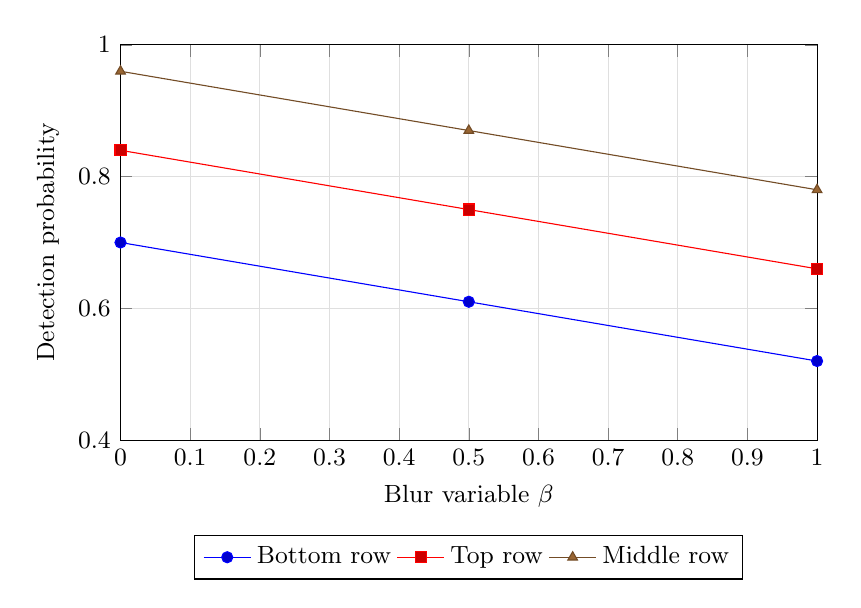
\begin{tikzpicture}
\begin{axis}[
  width=0.86\textwidth,
  height=6.6cm,
  xlabel={Blur variable $\beta$},
  ylabel={Detection probability},
  ymin=0.4, ymax=1.0,
  xmin=0, xmax=1,
  legend style={font=\small, at={(0.5,-0.24)}, anchor=north, legend columns=3},
  tick label style={font=\small},
  label style={font=\small},
  grid=major,
  grid style={gray!25}
]
\addplot+[mark=*] coordinates {(0,0.70) (0.5,0.61) (1,0.52)};
\addplot+[mark=square*] coordinates {(0,0.84) (0.5,0.75) (1,0.66)};
\addplot+[mark=triangle*] coordinates {(0,0.96) (0.5,0.87) (1,0.78)};
\legend{Bottom row, Top row, Middle row}
\end{axis}
\end{tikzpicture}
\caption{Detection probability~\eqref{eq:detprob} against blur, for a stack tall enough to have a distinct bottom, middle, and top. The gap rule is asked to repair the bottom curve, not the middle one.}
\label{fig:detprob}
\end{figure}

On a front face of four rows and three columns with every cell occupied, twelve crates, the expected number of misses at $\beta=0$ is
\begin{equation}
3(1-0.70)+3(1-0.84)+6(1-0.96)
= 0.90+0.48+0.24
= 1.62.
\label{eq:expected-miss}
\end{equation}
At $\beta=1$ the same sum is $3(0.48)+3(0.34)+6(0.22)=3.78$. A middle miss is the miss the two-neighbor rule is built to restore: the cell above and the cell below exist. A bottom miss has no lower neighbor. It is restored only when both lateral neighbors were detected, which on a three-column bottom row is true for the middle cell and only half-supported for the two ends. The rule is therefore a better repair of an interior hole than of a shadowed corner. Equation~\eqref{eq:expected-miss} says there is about one and a half misses to repair on a clean frame of that size, and nearly four on a blurred one. False positives arrive at a Poisson mean of $0.35$, an order of magnitude smaller than the blur-induced misses and large enough, across five independent frames, to supply the phantom cells that PLC-passage unions. The asymmetry is the design reason for trusting one frame.

The expected miss count is not the expected counting error. A miss that the gap rule restores costs nothing. A miss at a corner that the rule cannot see costs $\hat{d}$. A false positive that lands in an empty cell and acquires a second neighbor costs $\hat{d}$ the other way. The tables in Chapter~\ref{ch:system} are the net of those three effects. The expectation~\eqref{eq:expected-miss} only explains why the net is not zero and why it depends on which row was lost.

\subsection{The worked grid, drawn}
\label{sec:grid-drawn}

\Cref{fig:grid} draws~\eqref{eq:example-grid} before and after the pass~\eqref{eq:gap}. The occupied cells are the ten true front crates. The cell that the rule adds is the middle of the top row, which has a neighbor below and a neighbor to the right. The corner cell of that row has, at the moment it is visited, only the neighbor below, so it stays empty. The drawing is the whole of the positive bias on this stack: one invented front cell, times a depth of two, is two invented crates, before any missed detection is put back. When the first frame of the instrument also misses one true cell and the rule restores it, the invented cell remains and the declared front occupancy is eleven. Eleven times two is the $22$ reported later against a truth of $20$.

\begin{figure}[t]
\centering
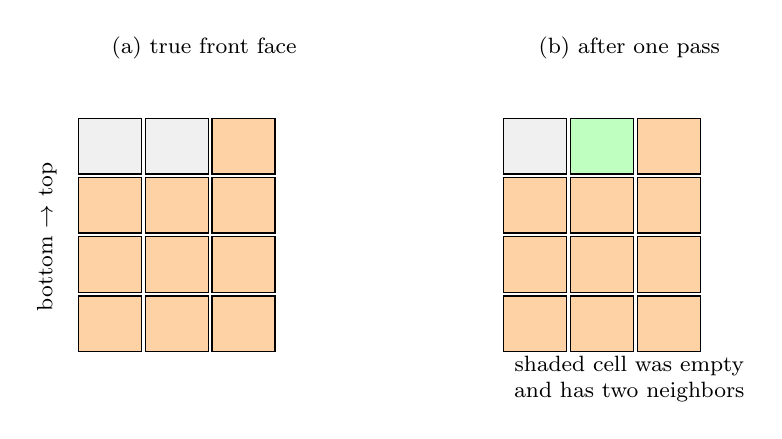
\begin{tikzpicture}[
  font=\footnotesize,
  c/.style={draw, minimum width=8mm, minimum height=7mm, inner sep=0pt, anchor=center},
  on/.style={c, fill=orange!35},
  off/.style={c, fill=black!6},
  add/.style={c, fill=green!25}
]
  \node at (1.2,3.5) {(a) true front face};
  \foreach \r in {0,1,2} {
    \foreach \col in {0,1,2} {
      \node[on] at (\col*0.85, \r*0.75) {};
    }
  }
  \node[off] at (0, 2.25) {};
  \node[off] at (0.85, 2.25) {};
  \node[on] at (1.70, 2.25) {};
  \node[rotate=90, anchor=south] at (-0.55,1.1) {bottom $\rightarrow$ top};

  \begin{scope}[shift={(5.4,0)}]
    \node at (1.2,3.5) {(b) after one pass};
    \foreach \r in {0,1,2} {
      \foreach \col in {0,1,2} {
        \node[on] at (\col*0.85, \r*0.75) {};
      }
    }
    \node[off] at (0, 2.25) {};
    \node[add] at (0.85, 2.25) {};
    \node[on] at (1.70, 2.25) {};
    \node[align=center] at (1.2,-0.7) {shaded cell was empty\\and has two neighbors};
  \end{scope}
\end{tikzpicture}
\caption{The stepped stack of the worked example. The top row truly contains one crate. Gap completion fills the cell beside it and does not fill the corner, because the corner is visited first and has only one orthogonal neighbor at that moment.}
\label{fig:grid}
\end{figure}

The order dependence is visible in the drawing and is easy to overstate. If the pass visited columns from right to left, the middle top cell would still have its lower neighbor and its right neighbor, both original, and would still be filled. The corner would then be visited after the middle cell existed, and would gain a lateral neighbor. A right-to-left pass would fill both empty cells. The implementation visits left to right and therefore fills one. This is a reason to treat the threshold and the visit order as part of the algorithm that was estimated, not as a cosmetic of the pseudocode. A later change to the visit order is a different counter and needs its own row in the table. The present row is the left-to-right, immediate-update, threshold-two counter.

\subsection{A bound on a single false center}
\label{sec:false-center}

One false center can do only a limited amount of damage on a single frame, which is the other half of the argument against the passage union. Suppose the true occupied set is a solid rectangle and the origin is exact. A false center falls either in an occupied cell, in which case the snap ignores the duplicate, or in an empty cell. An empty cell adjacent to the rectangle has at most one orthogonal neighbor inside the rectangle if it shares a side, and it has none if it only touches a corner. The test $n\ge 2$ does not add a side-adjacent cell on the strength of one false center. The false center occupies a cell by itself, and the count grows by $\hat{d}$, once. It does not start a rind.

The passage union removes that limit. Frame $1$ may place a false center on the left of the rectangle and frame $2$ a false center above that false cell, or two frames may place false centers in the same empty side cell and in a second empty cell that becomes its neighbor through the immediate update. Vote threshold one treats each of those as support. The single-frame bound, ``one false center adds at most one cell,'' is false of the union. The estimated bias of $+5.33$ crates for PLC-passage against $+0.83$ for PLC-single is the bound failing in the direction the mechanism predicts. It is also the reason the software specification has no vote accumulator. An accumulator with threshold one is not a harmless extra. It is the counter the estimate rejected.

\subsection{Why the span is the serious baseline}
\label{sec:span-serious}

The mask tally and the area ratio are easy to beat once depth is multiplied in, and a comparison that stopped there would overstate the lattice. The span is the serious baseline because it already knows $(w,h)$ and it already refuses to count raw detections. The three tenths of a crate that separate PLC-single from the span are the entire geometric contribution of the neighbor test, and they should be described at that size.

On a solid rectangle whose corner crates were detected, the span's percentile width and height recover the true number of rows and columns, and the span books $d$ times that product. PLC books the same product if every interior hole was restored and no phantom was added. The two counters differ when the outline is not a solid rectangle, when a false center stretches a percentile, or when an interior miss is common and the span, which does not look inside the rectangle, cannot tell a hole from a filled cell. The stepped top row is the first case. A false center just outside the left column is the second: the second percentile of $x$ moves, $\hat n_c$ in~\eqref{eq:span} can increase by one, and the span multiplies a whole extra column by the number of rows and by $\hat d$. PLC snaps that false center into one cell. If the cell has fewer than two neighbors it stays a single phantom, not a column. The neighbor test is a limit on how much one false center can inflate the count, which is the same limit Section~\ref{sec:false-center} stated from the other direction, and it is the reason a method with a slightly higher exact-match rate can still be the one to deploy when the alternative's errors come in whole columns.

None of this makes the span a straw man. On the loads the generator actually draws, most faces are nearly solid, the span's mean absolute error is $3.31$ against PLC-single's $3.01$, and a deployer who implemented only the span would have captured most of the gain over mask-times-depth. The thesis still specifies the neighbor test, because the extra code is a double loop over a few dozen cells, because the bias drops from $+1.60$ to $+0.83$, and because the failure mode of an extra column is worse than the failure mode of a single phantom cell on a step. The specification would be different if the estimate had gone the other way. It did not.

\begin{figure}[p]
\centering
\begin{tikzpicture}[
  font=\small,
  box/.style={draw, rounded corners=2pt, align=center, inner sep=5pt, minimum width=32mm, minimum height=12mm},
  arr/.style={-{Stealth}, thick}
]
  \node[box, fill=black!6] (det) {Detections\\$m_{\star}-q+f$};
  \node[box, fill=green!15, right=14mm of det] (rule) {Gap rule\\$+r$ restorations\\$+p$ phantoms};
  \node[box, fill=orange!15, right=14mm of rule] (front) {Front count\\$m$};
  \node[box, fill=blue!10, below=16mm of front] (book) {Booked total\\$\hat d \cdot m$};
  \node[box, fill=red!8, left=14mm of book] (depth) {Depth reading\\correct, or $\pm 1$};
  \node[box, fill=black!4, left=14mm of depth] (truth) {Truth\\$N=d\,m_{\star}$};
  \draw[arr] (det) -- (rule);
  \draw[arr] (rule) -- (front);
  \draw[arr] (front) -- (book);
  \draw[arr] (depth) -- (book);
  \draw[arr, dashed] (truth) -- (book);
  \node[align=center, font=\footnotesize] at ($(det.south)+(0,-0.9)$) {misses $q$,\\false cells $f$};
  \node[align=center, font=\footnotesize] at ($(truth.south)+(0,-0.85)$) {signed error\\$\hat N-N$};
\end{tikzpicture}
\caption{How a booked count is assembled, in the letters of~\eqref{eq:front-signed}. The detector contributes misses and false cells. The gap rule puts some misses back and may add phantoms. Depth scales the front count and, when the reading is wrong, adds or removes a whole rank. The dashed arrow is the comparison the estimate computes. It is not an input to the system.}
\label{fig:balance}
\end{figure}


\subsection{How the two updates meet}
\label{sec:meet}

ICPH and PLC share the mask and nothing else. The mask provides pixels to the feature~\eqref{eq:feature} and a center to the snap~\eqref{eq:snap}. After that split, a color error and a count error are different events. The per-color count that \Cref{def:task} asks for is the combination
\begin{equation}
\hat{N}_{k}
= \hat{d}\;
\lvert\{ (r,c)\in\mathcal{F} : \hat{k}(r,c)=k \}\rvert,
\label{eq:per-color}
\end{equation}
where a completed cell that no detection owns inherits the color of the majority of its orthogonal neighbors, and a tie inherits the color of the neighbor with the larger margin. Inheritance is specified here and not estimated, because the Monte Carlo trials do not assign classes and cells in the same draw. The specification is the one a deployment would code. Its error, when a completed cell inherits a swapped amber label, is the sum of the two errors the estimate does measure. An upper bound that does not pretend to be tighter than the data is
\begin{equation}
\lvert\hat{N}_{k}-N_{k}\rvert
\le \lvert\hat{N}-N\rvert + E_{k},
\label{eq:bound}
\end{equation}
where $E_k$ is the number of front crates whose type was swapped into or out of class $k$, times $\hat{d}$ if the depth reading was applied to both. The bound says that type errors and count errors add. It does not say they cancel. The system reports them as separate lines so that a cancellation in the total cannot hide a swap in the colors.

The two updates are also independent in their requirements. ICPH needs \Cref{ass:color} and a mask that overlaps the face. PLC needs \Cref{ass:lattice}, a homography, and a depth reading. A building that controls its lamps and not its geometry would enable PLC and could turn ICPH down to the raw matcher. A building that has irregular mixed cartons and stable lamps would do the opposite, and would leave this thesis's lattice behind in favor of the area ratio. The brewery passage, as defined in Section~\ref{sec:scene}, enables both, which is why both are in the updated model.

The updated model, named in full, is YOLO-vf-seg with the vertical-feature neck~\eqref{eq:vf}, the prototype mask assembly~\eqref{eq:yolact}, the chromatic head of \Cref{alg:feature} and~\eqref{eq:linear}, and the lattice counter of \Cref{alg:plc}. The next chapter places that model in the passage: where the camera stands, what the computer stores, how a frame becomes a line on the operator's tally, and what the Monte Carlo estimate says about the head and the counter when the passage is simulated rather than filmed.
